This chapter will discuss the process of implementing the application. The justification of the technologies and processes used, along with the benefits, and challenges they potentially presented will be discussed here.

\section{Version Control}
Version control is required to have been used throughout the duration of the project. Version control allows a developer to keep track of and manage changes made to source code and other software artefacts during development. Good utilization of version control is critical to the success of a project and helps to keep a project organised.
\subsection{GitHub \& Git}
GitHub \cite{github} is a platform widely used throughout the industry to store software projects online. GitHub allows users to create Git repositories \cite{git} that contain files used within a project, along with their version history. This combination of Git and GitHub is widely used within the industry due to the distributed nature of version control, and the various tools offered by GitHub to enhance the developer experience. Both these tools were very familiar, so this made Git, and GitHub a simple choice. 
\subsubsection{Feature Branching}
An advantage of using a distributed version control system such as Git, is how easy branching is due to the easy creation of multiple local branches. Feature branching was used throughout this project (see \ref{fig:branching}), with features developed in local feature branches, then merged back with the main branch upon completion.  
\begin{figure}[!htbp]
    \centering
    \begin{subfigure}[b]{0.90\textwidth}
        \frame{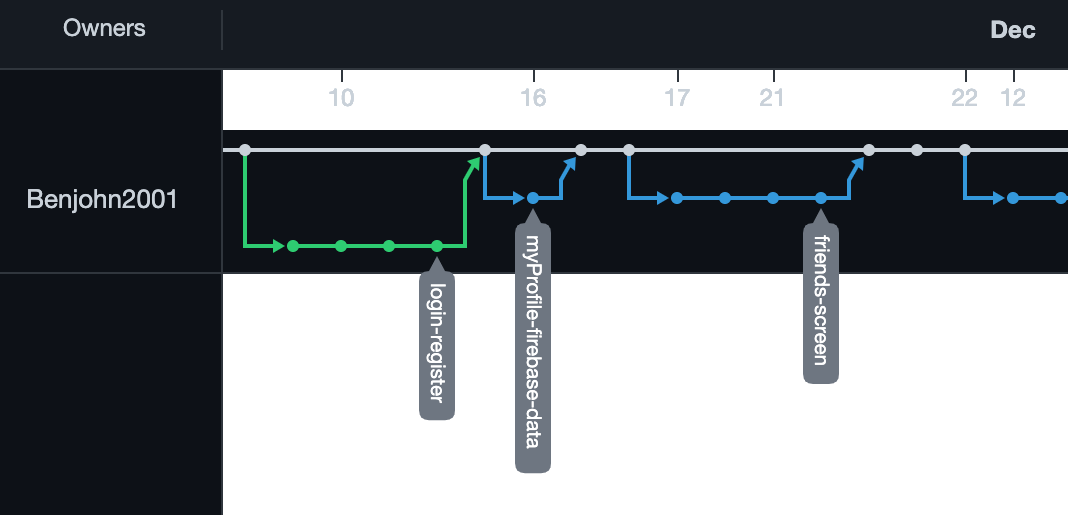
\includegraphics[width=\textwidth]{featureBranch.png}}
    \end{subfigure}
    \caption{Example of feature branching used in the project}
    \label{fig:branching}
\end{figure}
\subsubsection{Issue Tracking}
The GitHub issue tracker was used to keep track of outstanding tasks, along with any bugs that needed to be fixed. GitHub allows the addition of labels to issues helping the developer separate concerns, such as Firebase and design issues for example (see \ref{fig:issues}).
\begin{figure}[!htbp]
    \centering
    \begin{subfigure}[b]{0.90\textwidth}
        \frame{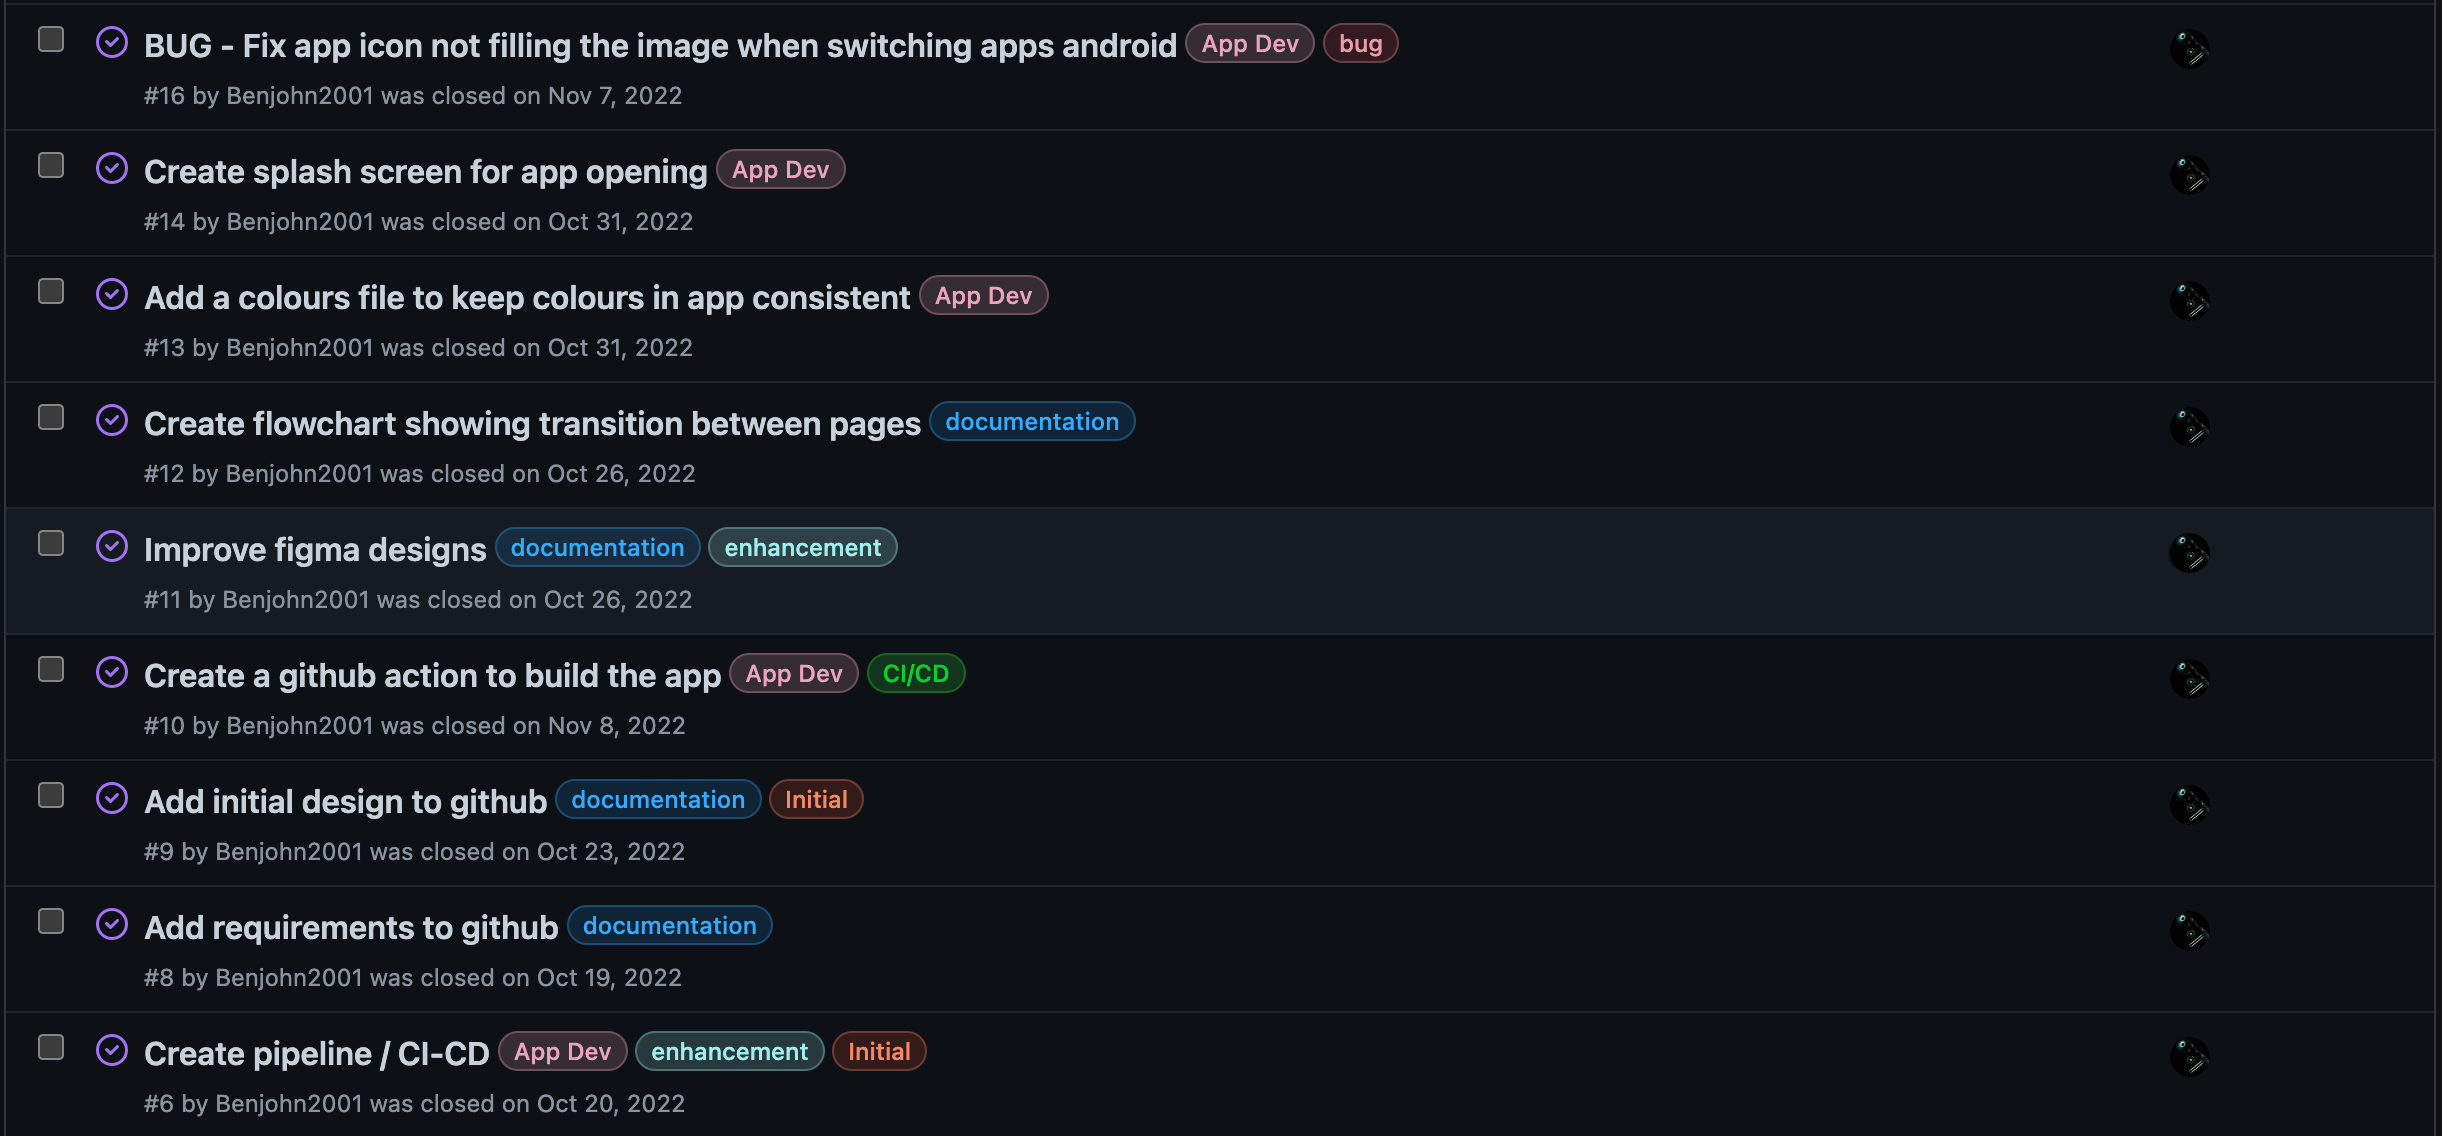
\includegraphics[width=\textwidth]{issues.png}}
    \end{subfigure}
    \caption{Examples of issues created in GitHub's issue tracker}
    \label{fig:issues}
\end{figure}
\subsubsection{Actions}\label{ghActions}
GitHub actions is a continuous integration and continuous delivery tool that allows the developer to create job workflows that can be triggered on specific behaviour. A workflow that built, and published the application upon a push to the main branch was created. This enabled the newest version of the application to be always accessible on a mobile device, allowing constant testing of new features to occur. A testing workflow was also created with pushes to the tests, or main branch running the test suite, along with code formatting, and style checks (see \ref{CodeF&S}).
\section{Technologies}
As mentioned in \ref{designDecis}, a comparative study \cite{compStudy} was performed in the early stages to help decide what technologies were best suited to the task. The technologies used to create the application will be discussed in this section.
\subsection{React Native}\label{reactSection}
When creating a mobile application there are two options, native applications for each operating system, or cross platform frameworks allowing a single code base to create applications for both operating systems. Whilst there are many advantages of native development such as the utilisation of many platform specific features, the development time of creating two consistent, but separate apps was simply infeasible within the time constraints. React Native \cite{reactnative} allows the creation of applications using JavaScript \cite{js} in a singular code base. This was chosen over other alternatives due to the component-based nature and flexibility provided by the framework.
\subsubsection{Expo}
React Native development does however require some native coding and the presence of build tools for both operating systems. This meant that both Android Studio (Android IDE) and XCode (iOS IDE) would both have to be installed on the device used for developing the application, which was an issue due to low storage space. Due to no native coding being required in this project the choice to use Expo \cite{expo}, a framework designed to ease the creation of React Native applications was made. Expo requires no native coding, or build tools allowing developers to simply run a command in the terminal to build, and access the application on a personal device, or emulator.
\begin{figure}[!htbp]
\centering
\begin{subfigure}[b]{0.5\textwidth}
\begin{lstlisting}[language=bash]
  $ expo start --ios
  $ expo start --android
\end{lstlisting}
\end{subfigure}
\caption{To build and start applications with expo for iOS or Android}
\end{figure}
\subsection{Tailwind CSS}
When creating a user interface there are several CSS frameworks and UI kits that can be used in tandem, or independently of standard CSS style sheets. Tailwind CSS \cite{tailwind} is a CSS framework that allows the developer to apply styles to components by using given utility classes in the className property. Tailwind does not include styled components of their own giving full control to the developer over the design. This approach was chosen over a UI kit of predesigned components, allowing the design to be unique, and flexible to the project requirements. NativeWind \cite{nativewind} is a package used to process the CSS from the tailwind class names into StyleSheet objects, that can then be understood by React Native. The use of this technology enhanced the quality of the user interface, and developer experience by allowing full flexibility over design, and an easier, more flexible alternative to traditional CSS style sheets.
\begin{figure}[!htbp]
    \centering
    \begin{subfigure}[b]{0.42\textwidth}
        \begin{lstlisting}[language=jsJsx, caption={Styled using Tailwind CSS}]
        <TouchableOpacity
            onPress={onPressFunction}
            className="bg-darkerPurple h-12 w-10/12 rounded-full"
        >
            <Text className="text-white text-center">
                Press Me
            </Text>
        </TouchableOpacity>
        \end{lstlisting}
    \end{subfigure}
    \hspace{2em}
    \begin{subfigure}[b]{0.45\textwidth}
        \begin{lstlisting}[language=jsJsx, caption={Styled using a traditional StyleSheet}]
        <TouchableOpacity
            onPress={onPressFunction}
            style={styles.button}
        >
            <Text style={styles.text}>
                Press Me
            </Text>
        </TouchableOpacity>
            
        const styles = StyleSheet.create({
          button: {
            justifyContent: 'center',
            backgroundColor: 'purple',
            borderRadius: 9999,
            height:48,
            width:200,
          },
          text: {
            textAlign: 'center',
            color: 'white'
          },
        });
        \end{lstlisting}
    \end{subfigure}
    \caption{Example of a simple styled button}
    \label{fig:tailwind}
\end{figure}
\FloatBarrier
\subsection{Code Formatting \& Style} \label{CodeF&S}
To ensure the code was consistent and free of bugs, the code formatter Prettier \cite{prettier}, and code analysis tool ESLint \cite{eslint} were used. Prettier rewrites code into a consistent style, ensuring all files in the code base are formatted consistently, and correctly. ESLint is a linter for JavaScript that analyzes code finding errors and enforcing a chosen code style. Airbnb \cite{airbnb} code style was chosen for this project being the most popular JavaScript style guide. Both these tools were used together to ensure bug free, consistent, and readable code. 
\subsection{Firebase}\label{firebaseSection}
To store and authenticate data access for the application, Google's Firebase \cite{firebase} platform was chosen. Firebase allows developers to have real-time access to their hosted services from the client-side code. Firebase was chosen due to being optimised for mobile applications with real-time NoSQL \cite{nosql} databases, and many other helpful services. Although Firebase has a paid tier, the free tier would suffice for this project's requirements.     
\subsubsection{Authentication}
Firebase provides an authentication service allowing the application to verify the identity of users. The service is easy to set up and use alongside other Firebase services. Firebase's authentication service is also very secure due to being maintained by Google.
\subsubsection{Storage}
Firebase cloud storage was used to store the images used throughout the application. Storage of these images was easy to implement with paths to the images being stored in the database, and the images themselves securely uploaded and downloaded from the cloud storage when required.
\subsubsection{Realtime Database}
The application data is stored in a NoSQL, cloud hosted database through Firebase's realtime database service. This allows for real-time syncing of data keeping the application up to date with any changes made. This requires no server setup and is relatively easy to manage, and scale.
\begin{figure}[!htbp]
\centering
\begin{subfigure}[b]{0.85\textwidth}
\begin{lstlisting}[language=json]
"KKSw9RsMRlSBKjUy7EGOiA1NcFk2": {
    "bio": "Im ben who shops at iceland",
    "email": "benjohnston2001@icloud.com",
    "firstName": "Ben",
    "lastName": "Johnston",
    "profilePic": "images/profilePics/KKSw9RsMRlSBKjUy7EGOiA1NcFk2",
    "userName": "Benjohn2001"
  },
\end{lstlisting}
\end{subfigure}
\caption{How data is stored in the Realtime Database as JSON objects.}
\small\par\textit{{The key "KKSw9RsMRlSBKjUy7EGOiA1NcFk2", is used to access this object in the database, and the user data, including the path to the user's profile picture stored in cloud storage.}}
\label{jsonResp}
\end{figure}

\section{Final Product}
The final product produced provides the user with an easy to use, and elegant application encompassing all of the must, and should have requirements. The application uses a consistent design throughout paired with an intuitive navigation system to make the application easy to learn and use. Users can register for an account, add their friends, then create groups that they can use to track their friend's status on a graphical clock.
\subsection{User Interface}
Due to the high quality designs discussed in \ref{UIDesign}, the implementation of the user interface simply required translating these wireframe designs, into application code.
By exploiting react native's component-based architecture, reusable UI components were constructed and used throughout the application to streamline the implementation, whilst keeping the design consistent (see \ref{appendix:appScreens}).
\subsubsection{WCAG}
The web content accessibility guidelines \cite{wcag} are a set of accessibility guidelines created by the World Wide Web Consortium (W3C) \cite{w3c} outlining how to make web content more accessible for users with disabilities, and impairments. These guidelines also apply to mobile applications and are recommended by the UK government \cite{govWCAG} to help developers create more accessible mobile apps. Some examples of where effort was made to conform to these guidelines are detailed below.
\begin{figure}[!htbp]
    \centering
    \begin{subfigure}[b]{0.45\textwidth}
        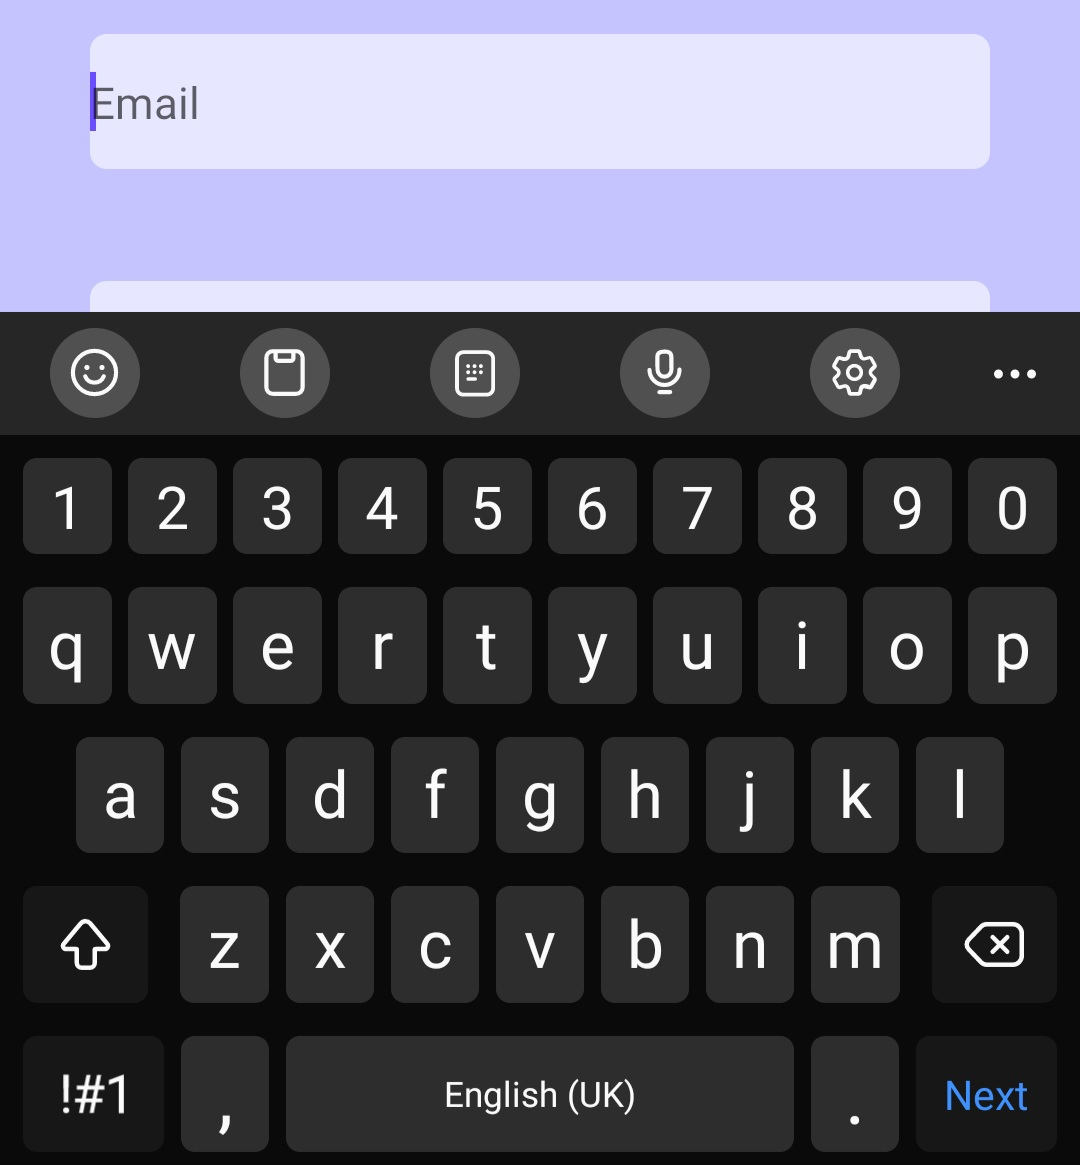
\includegraphics[width=\textwidth, height=5.5cm]{keyboard.jpg}
        \caption{\textbf{Keyboard \& Text Input:} The keyboard shifts focus onto the text input box when selected and allows navigation of the form by overriding the return key to `Next', and, `Done' \textbf{(Success Criterion 3.2.2)}. A cursor also highlights the current text box selected.}
    \end{subfigure}
    \hspace{1.5em}
    \begin{subfigure}[b]{0.45\textwidth}
        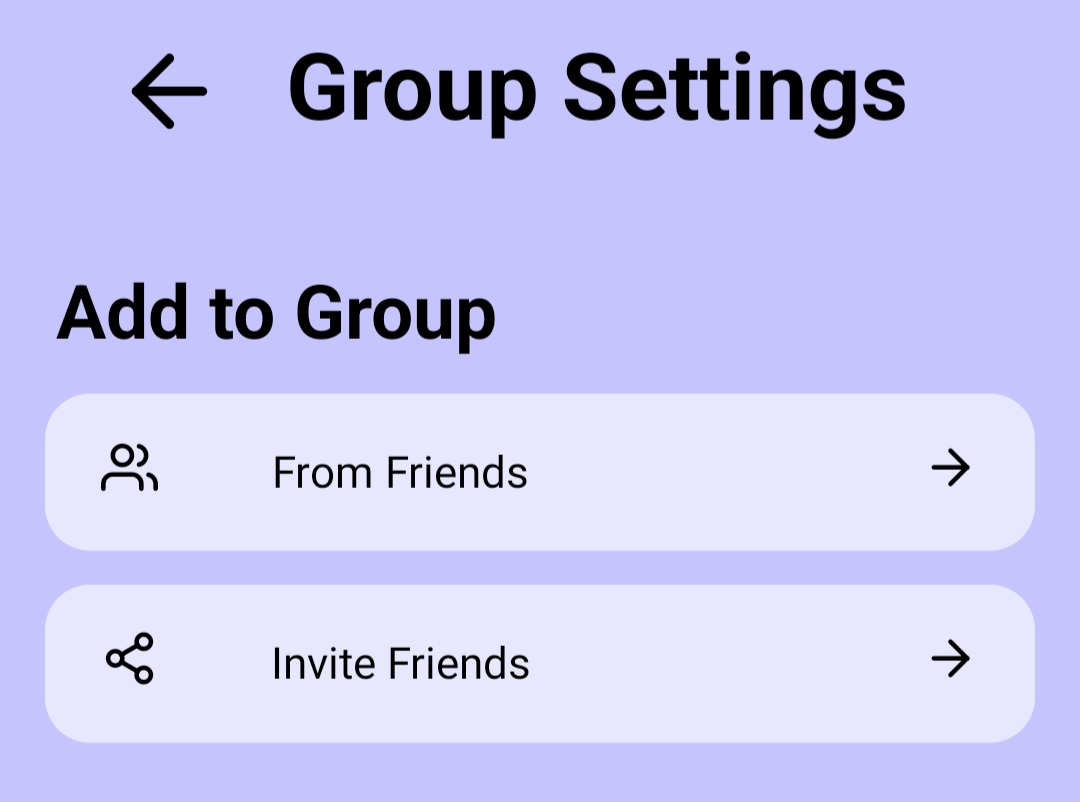
\includegraphics[width=\textwidth]{navigable.jpg}
        \caption{\textbf{Navigable:} Application screens have clear and consistent titles and navigation options helping users navigate, and determine their location. Headings are used to separate UI components making use of icons to help guide the user \textbf{(Success Criterion 2.4.2 \& 2.4.6)}.  }
    \end{subfigure}
    \vskip\baselineskip
    \begin{subfigure}[b]{0.45\textwidth}
        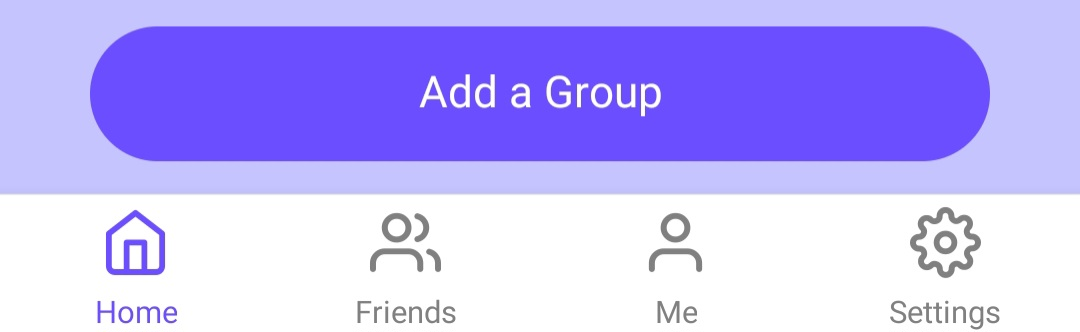
\includegraphics[width=\textwidth]{navbar.jpg}
        \caption{\textbf{Location:} The user's current location is displayed within the navigation bar \textbf{Success Criterion 2.4.8} }
    \end{subfigure}
    \caption{Examples of accessibility conformance throughout the application}
    \label{fig:accesibility}
\end{figure}
\FloatBarrier
\subsubsection{Nielsen's Heuristics }
In 1990 Jakob Nielsen created ten usability heuristics \cite{nielsen} to help designers create more usable interfaces. These heuristics were consulted when implementing the user interface, helping create a greater user experience. A navigation bar shows what page the user is currently on, and page headings help the user have visibility of system status. Recognition rather than recall is applied with the use of common icons throughout the application reducing the cognitive effort required by the user. The interface only displays the information needed by the user and has a minimalist design to not distract the user. Error messages are displayed in plain text form through alerts to the user so they can better understand errors, such as password restrictions. Providing users with a clear exit, and consistent design was also integral to the implementation, lowering the user's cognitive load, and keeping them in control. These heuristics along with the WCAG were considered throughout the implementation phase and helped to deliver a final product that was not only aesthetically pleasing but, usable.

\subsubsection{UI Implementation}
The user interface was created by having screens that would load the data from Firebase, and then present the data through custom, and core react native components. Reusable customized components were used throughout the application to display relevant data. These components have `props', which are the parameters used to pass data to be used in these components. These props can contain the data to be displayed, functions, or even icons and colours we would like to style the component with (see \ref{fig:reuseComp} for usage, and, \ref{appendix:reusable} for component code).


\begin{figure}[!htbp]
    \centering
    \begin{subfigure}[b]{0.25\textwidth}
        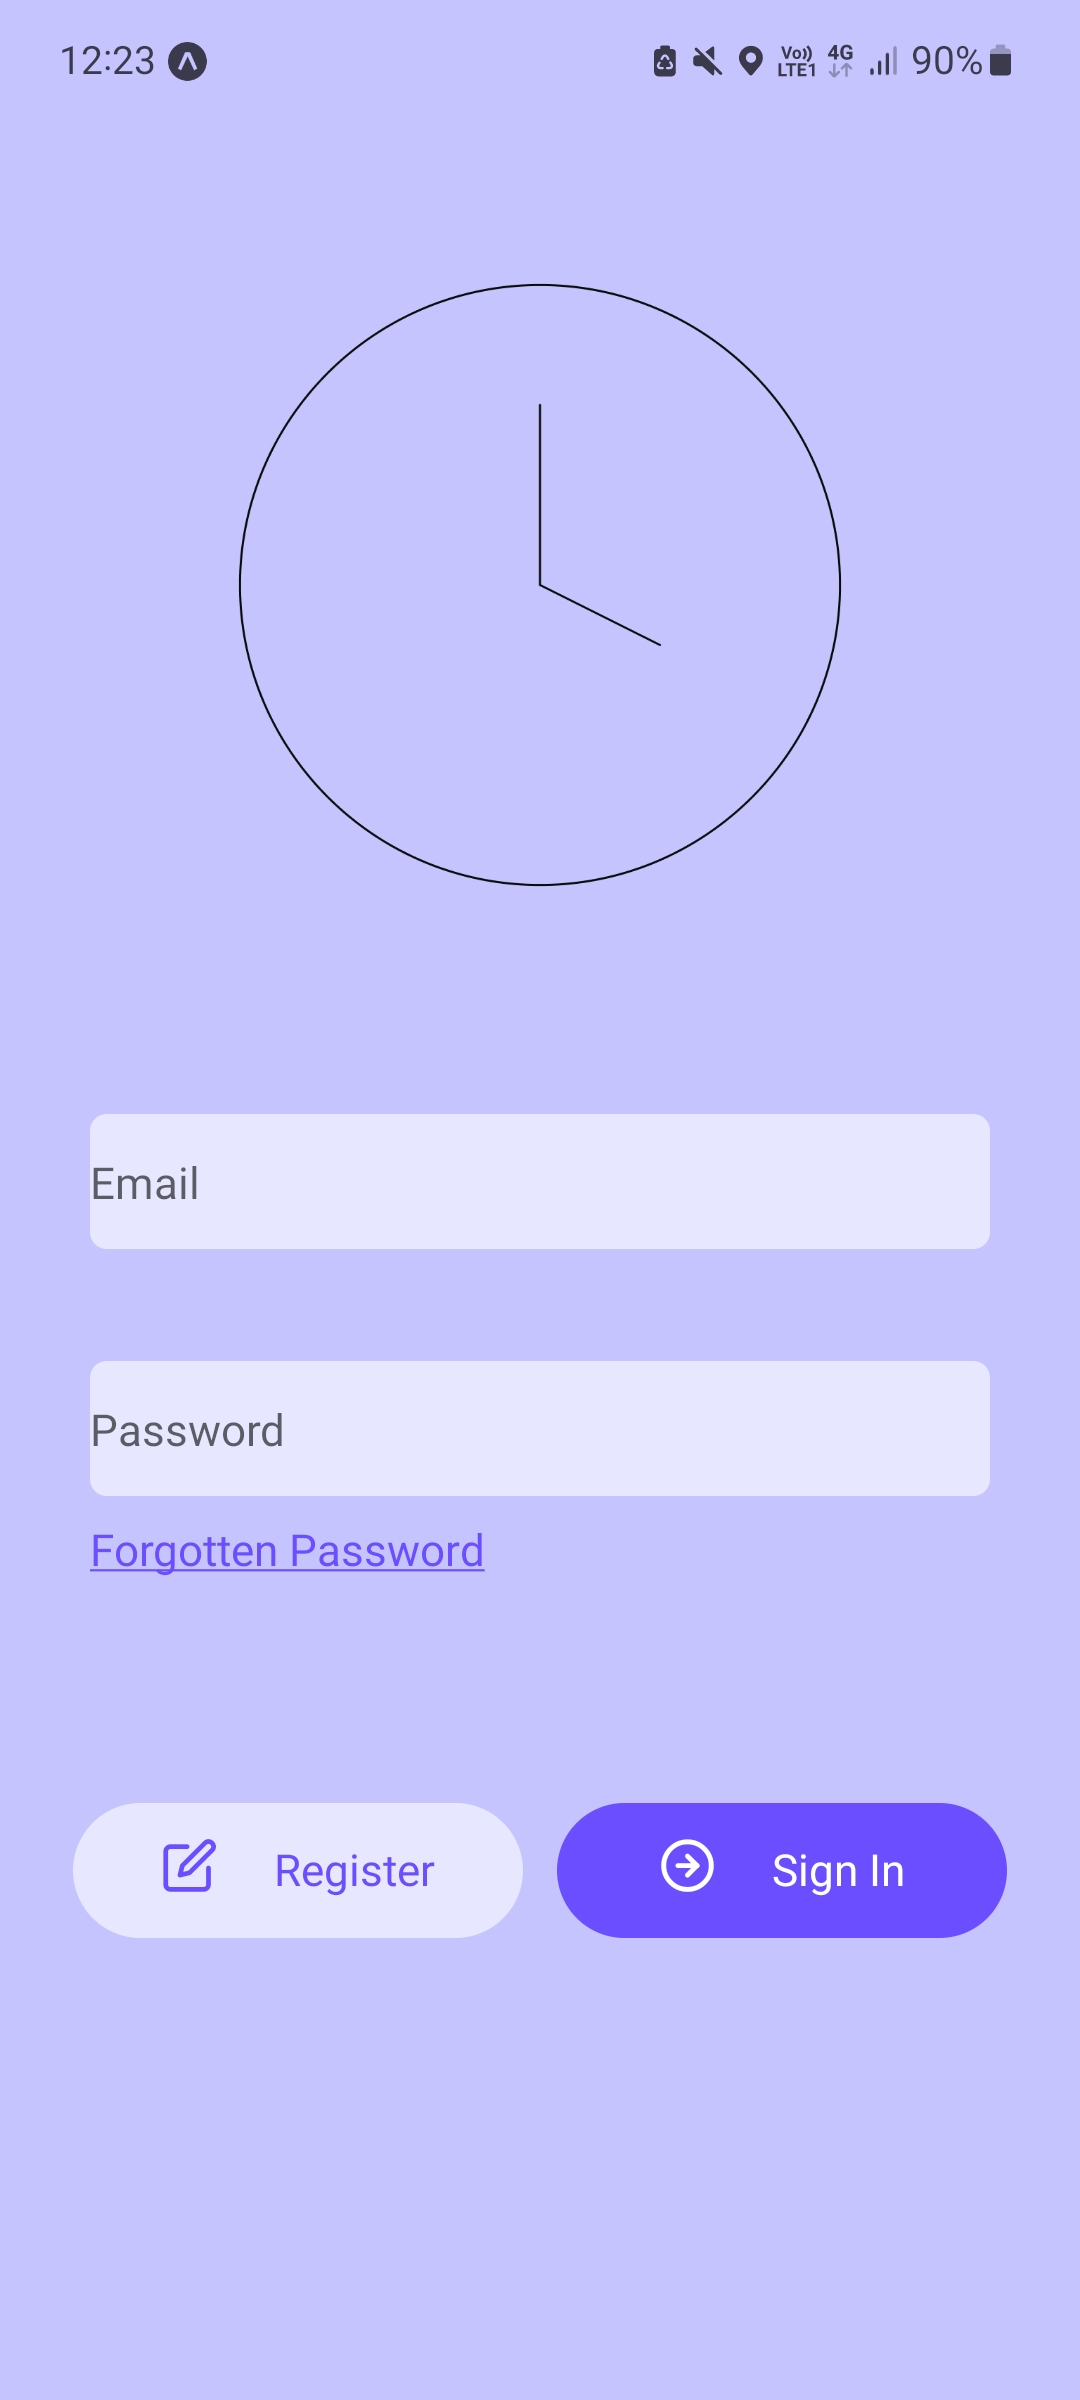
\includegraphics[width=\textwidth]{signIn.jpg}
        \caption{Register and Sign In buttons on Sign In page}
    \end{subfigure}
    \hspace{1.5em}
    \begin{subfigure}[b]{0.25\textwidth}
        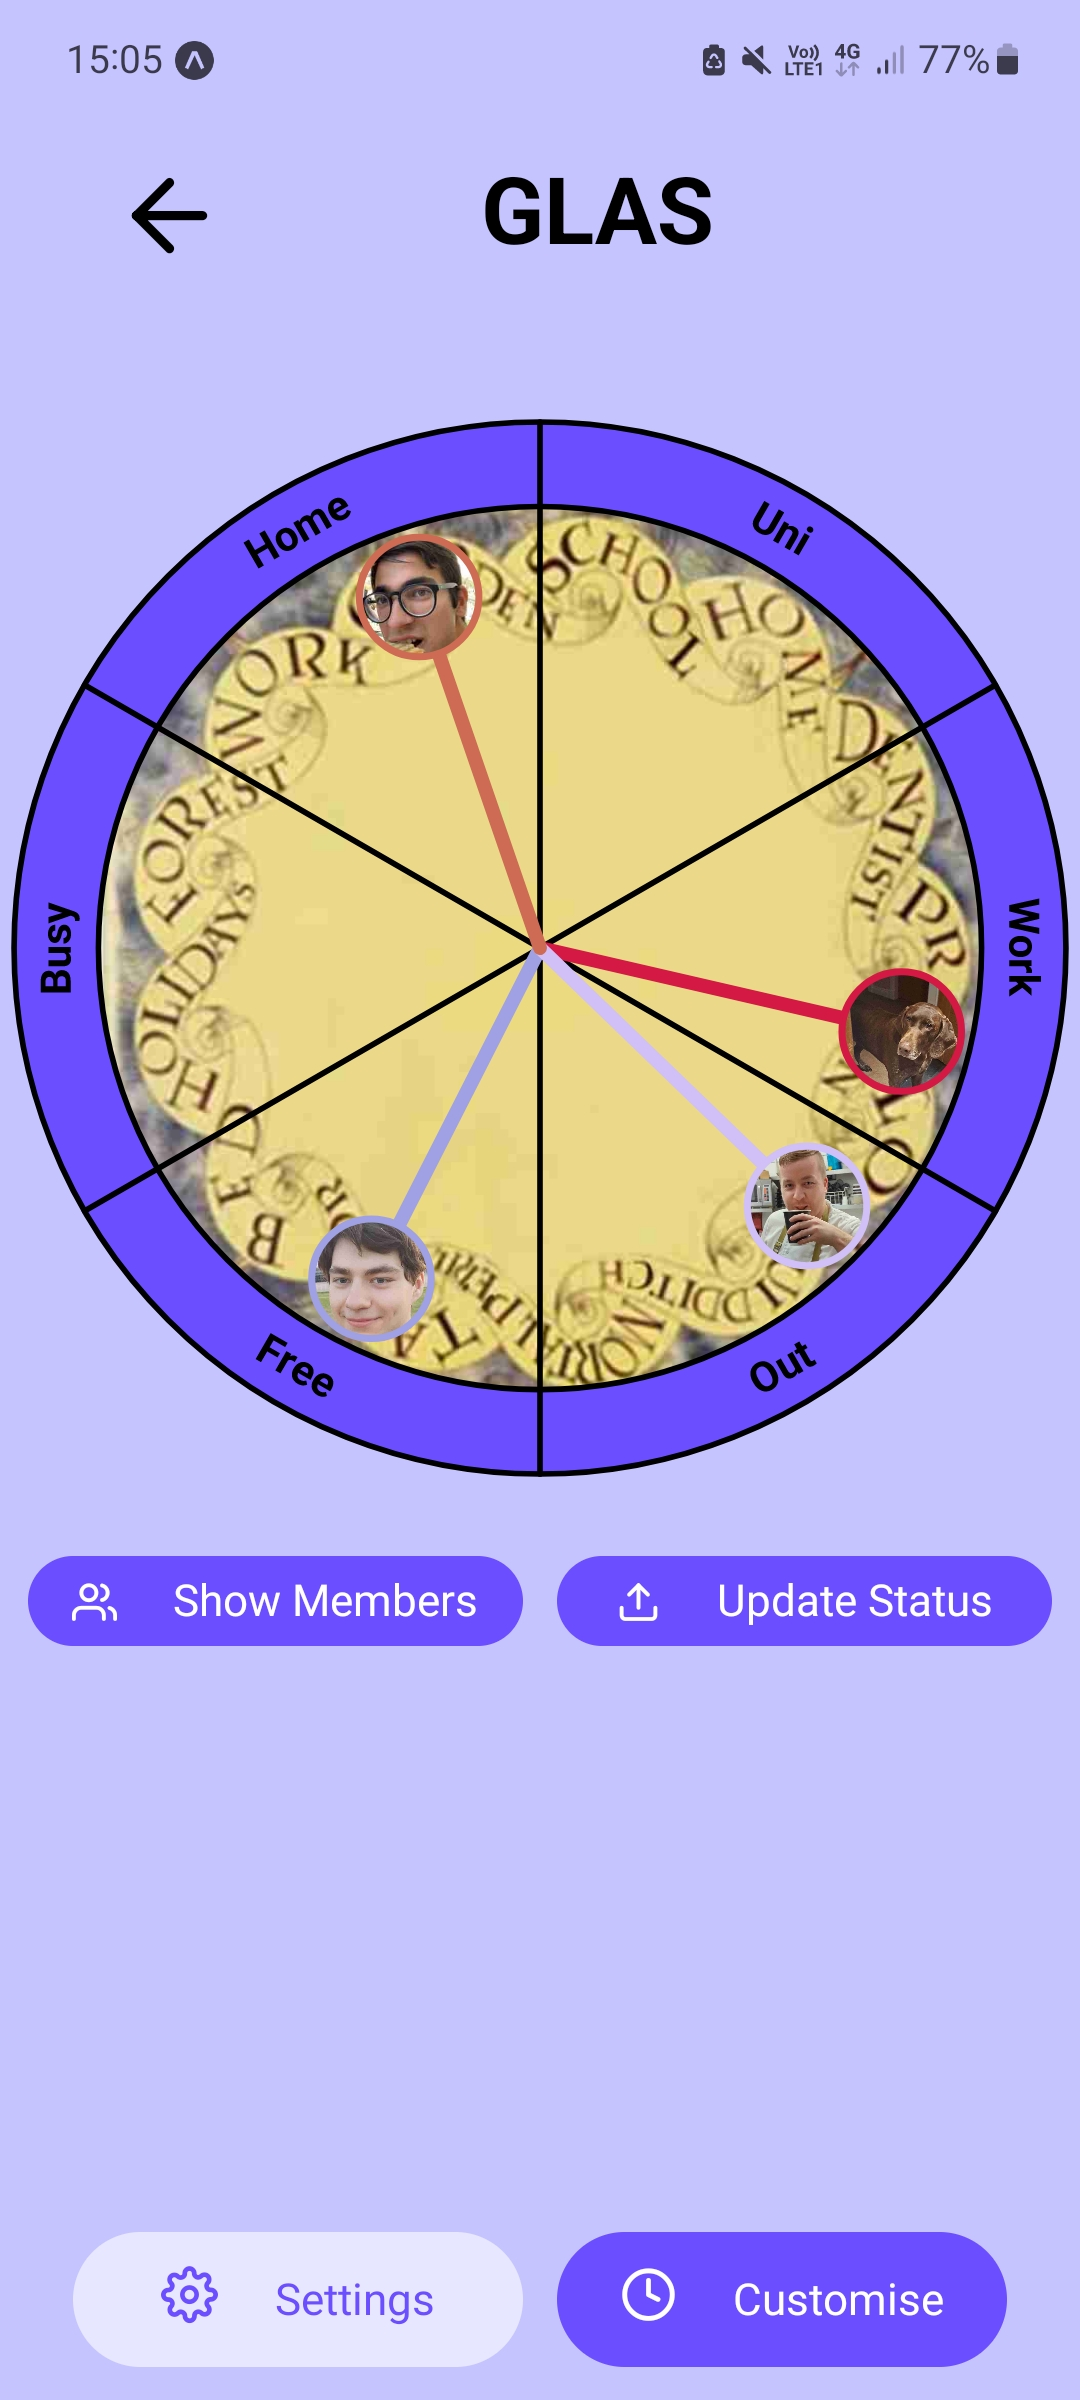
\includegraphics[width=\textwidth]{clock.jpg}
        \caption{Settings and Customise buttons on Group page}
    \end{subfigure}
    \caption{Example reuse of TwoButtonSide Component}
    \label{fig:reuseComp}
\end{figure}
\FloatBarrier
\subsection{Back End of Application}
As discussed in \ref{firebaseSection}, Firebase was used to store and manage all the data for the application, including graphics, and authentication. Firebase realtime database is a NoSQL database architecture storing data as objects in a JSON tree, as shown in figure \ref{jsonResp}. As discussed in \ref{dataMedStor}, nesting data is not an efficient or recommended practice, so instead, our data was separated into JSON objects representing subsections of the data. Application data was stored in the JSON objects users (user data), clockFace (clock background), friends (a user's friends list), groupMembers (a group's members), groups (a user's groups), and locations (storing a groups locations) (see \ref{appendix:rtdb}). As we are unable to store images in the realtime database, image paths were stored, then used to download the image when needed from cloud storage. User images were stored by a unique user id allowing easy fetching and deletion, along with ease of updates due to old images simply being overwritten. Email and password were used to create accounts and authentication data. Firebase authentication provided easy-to-use SDKs facilitating sign in, forgotten password, and registration of new users. This authentication data was also used to allow access to read, or write to the database and storage through security rules ensuring only authenticated users have access (see \ref{appendix:securityRulesRTDB} and \ref{appendix:securityRulesStor}). The sole use of Firebase throughout this project allowed the back end of the application to stay centralized within a sole platform, making it easier to implement and maintain. A diagram visualising the use of these Firebase services is shown below (see \ref{fig:firebaseDiag}).
\begin{figure}[!htbp]
    \centering
    \begin{subfigure}[b]{\textwidth}
        \frame{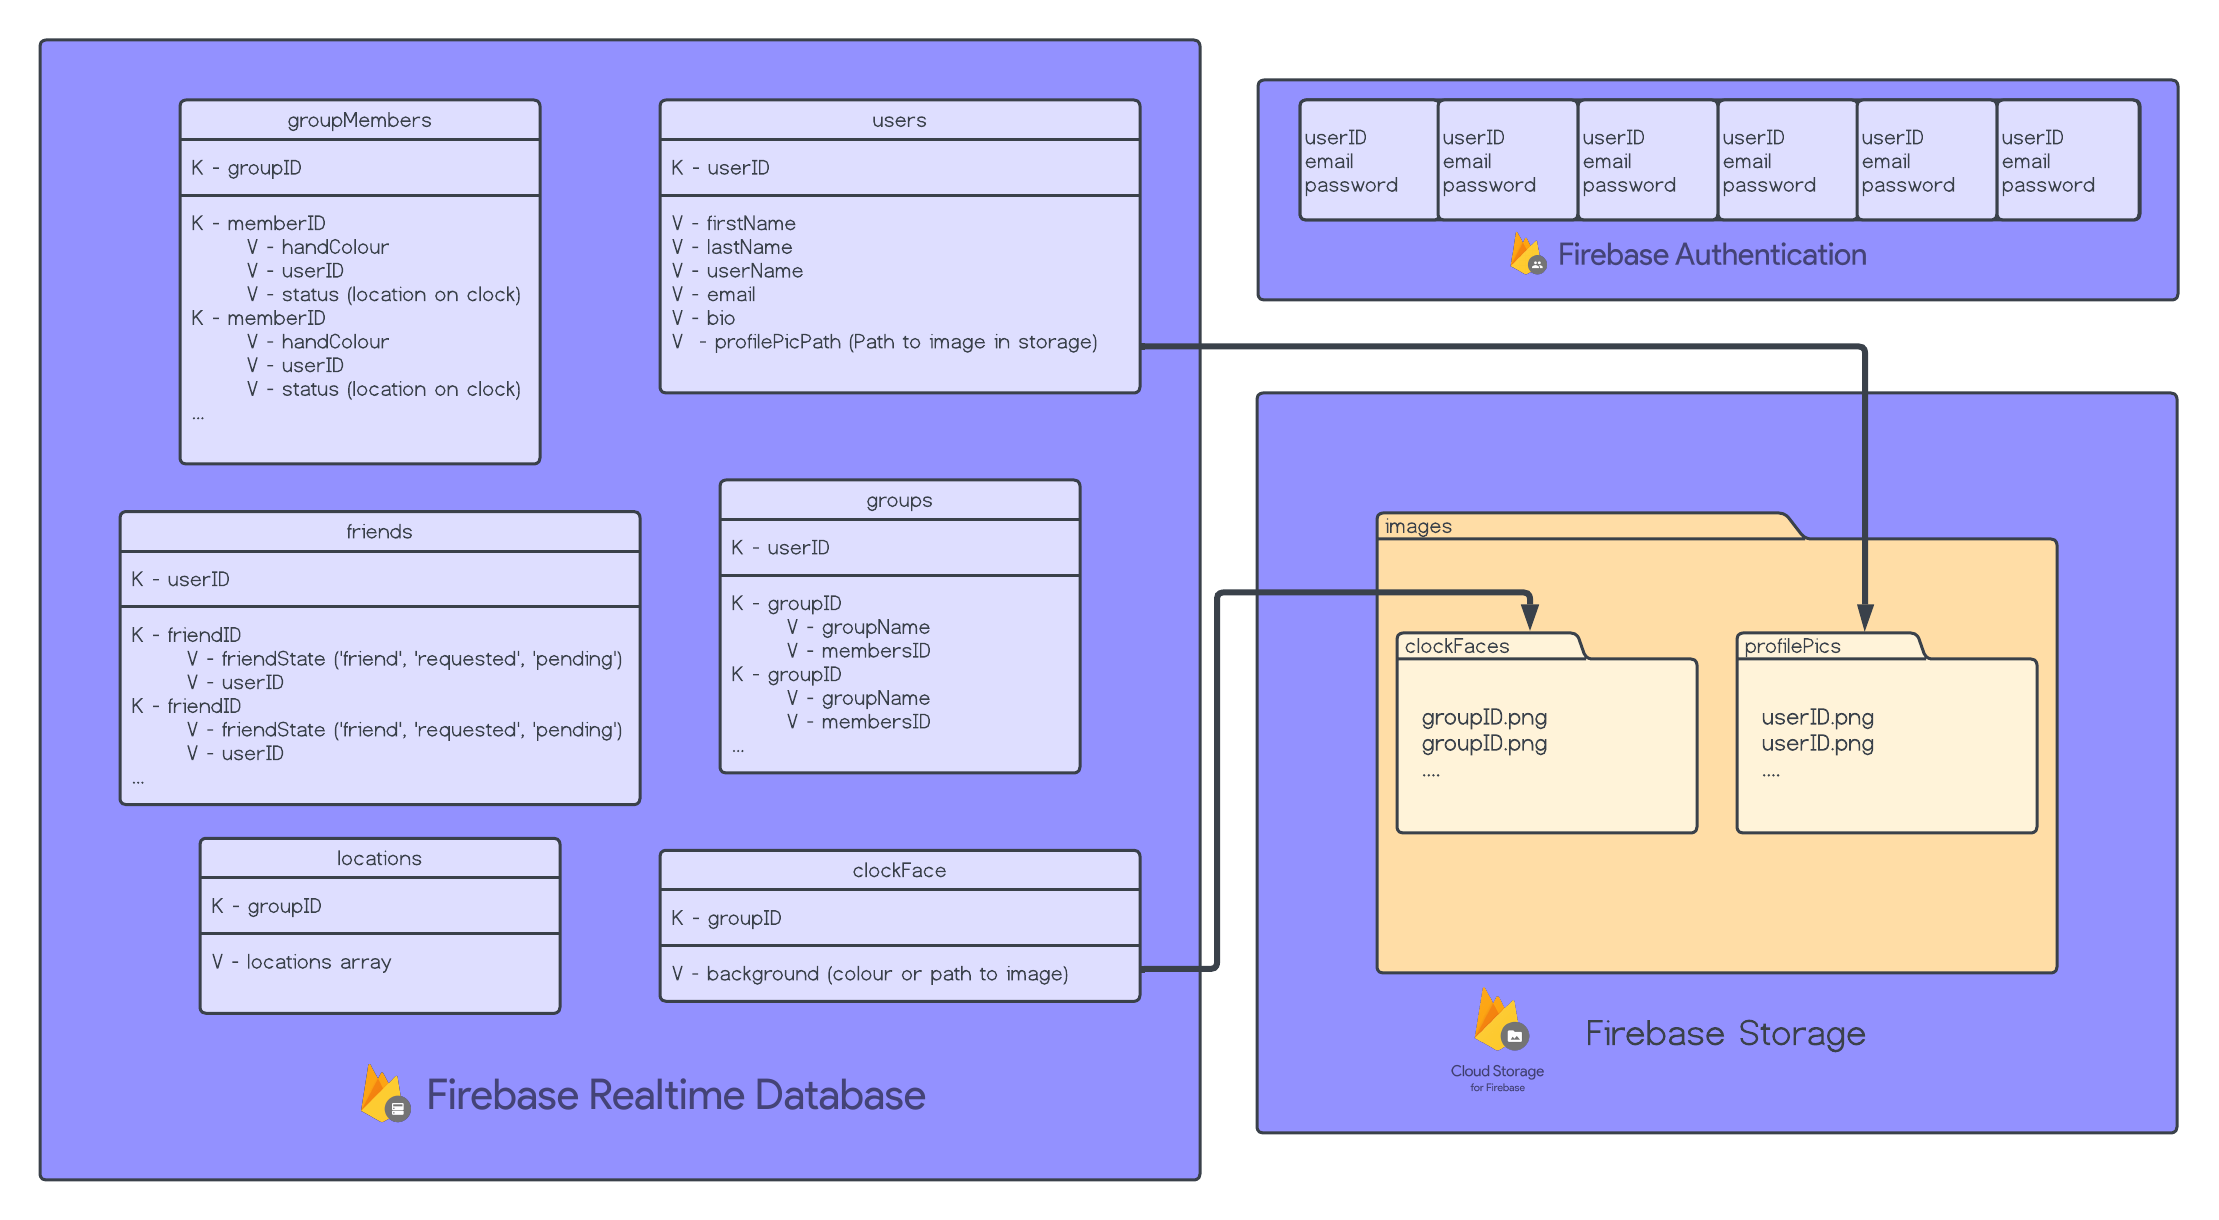
\includegraphics[width=\textwidth]{firebaseDiag.png}}
    \end{subfigure}
    \caption{Diagram visualising how data is stored in Firebase} \small\textit{{Logos: \cite{storImg, rtdbImg, authImg}}}
    \label{fig:firebaseDiag}
\end{figure}
\FloatBarrier
\section{Challenges}
Throughout implementation, many challenges were faced, and a few have been documented here.
\subsection*{Hand Placement}
After implementing the clock hand functionality, it was discovered that even while doing random hand placement in the statuses sector, if multiple users had all selected the same status, there was a significant hand overlap. This overlap presented issues for the user, making the clock difficult to interpret, a large issue. As these sectors could not simply be expanded due to a hard constraint of screen size, the approach of varying the length of the clock hand, along with random angles was taken to try and reduce this overlap. 
\vskip\baselineskip
\begin{algorithmic}[1]
\State $angle \gets randomAngleInSector$
\State $innerClockRadius \gets clockRadius-30$
\Comment{Subtract 30 to reach the inner clock, where the hands should be displayed}
\vskip\baselineskip
\If{$anotherMemberWithSameStatus$}
    \State $splitSpace \gets clockRadius / noOfMembers$ \Comment{Split radius into even chunks}
    \State $handLength \gets innerClockRadius - splitSpace * noOfMembersWithSameStatus $ \newline\Comment{Subtract enough chunks from the radius to fit the hand given the number of members with the same status }
\Else
    \State $handLength \gets innerClockRadius - 10$ 
    \Comment{Hand length is adjusted by 10 to ensure icon at the end of the hand fits inside the clock}
\EndIf
\end{algorithmic}
\vskip\baselineskip
First, a random angle in the sector is assigned to define the hand position, then the inner clock radius is set to ensure the hands fit inside the sector and do not cover the sector label. The hand length is then calculated by first checking whether another user has also selected that status, if so, the vertical space of the sector is split into even chunks. Then the number of members also choosing this status multiplied by this chunk value is subtracted to vary the length of the hands. If the user is alone in this sector, 10 units are subtracted from the hand length to ensure the clock hand icon also fits inside the sector. This approach is used to give the desired result reducing the overlap between hands as shown in \ref{fig:handPlacement} below.   
\begin{figure}[!htbp]
    \centering
    \begin{subfigure}[b]{0.33\textwidth}
        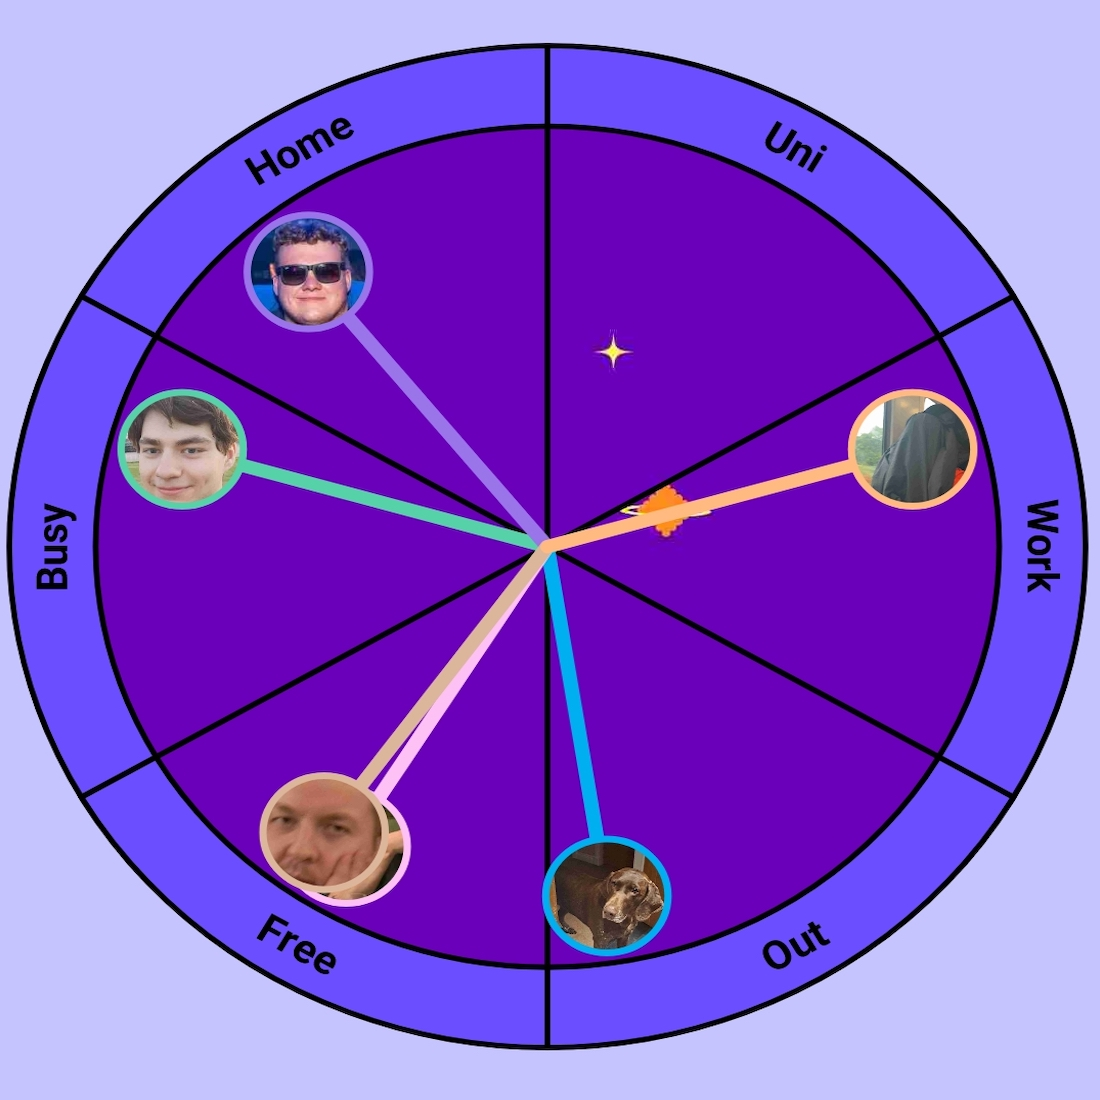
\includegraphics[width=\textwidth]{beforeHand.jpg}
        \caption{\textbf{Before:} Two hands overlapping in `Free'}
    \end{subfigure}
    \hspace{1.5em}
    \begin{subfigure}[b]{0.33\textwidth}
        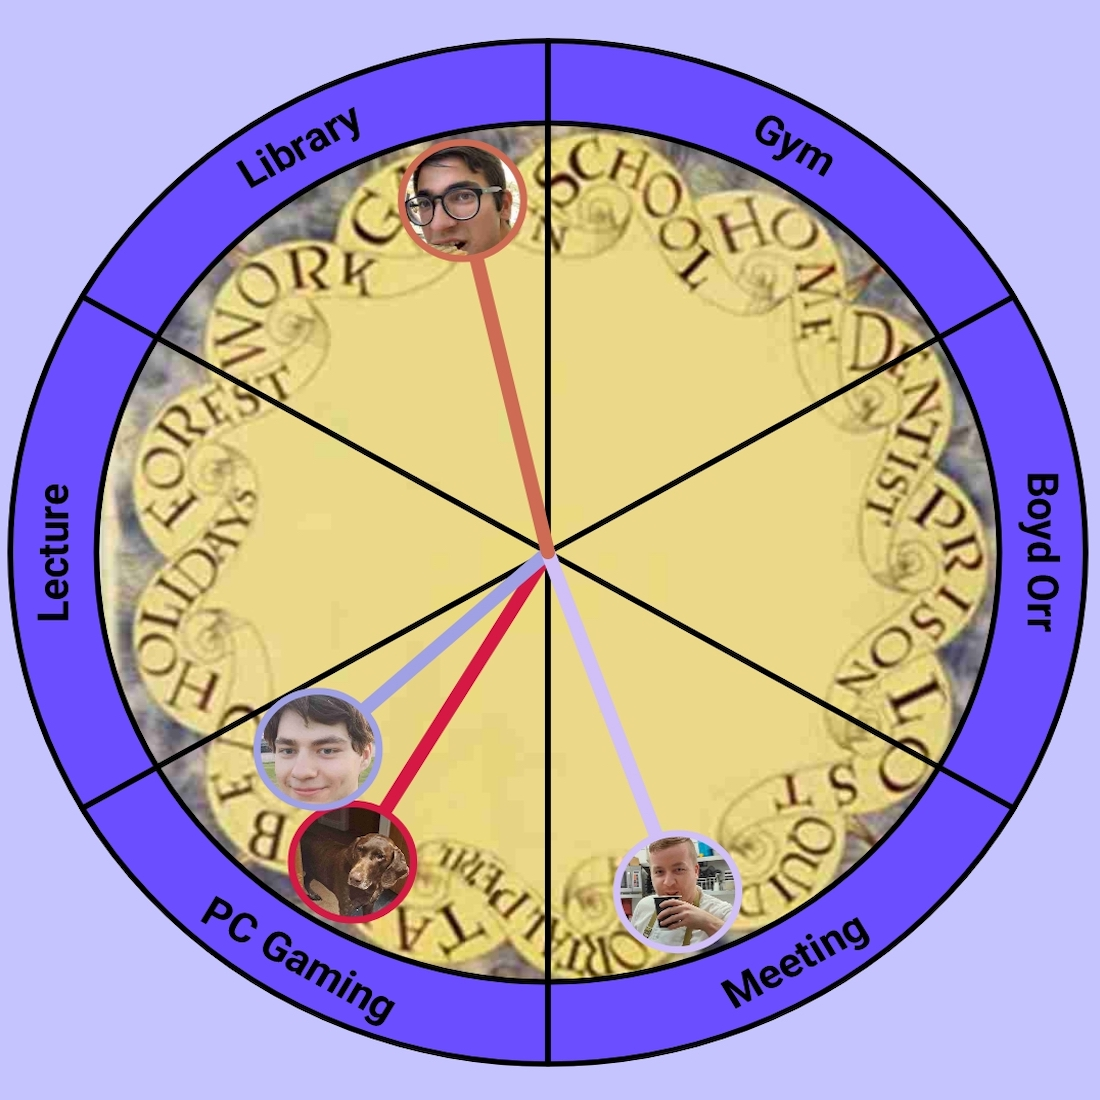
\includegraphics[width=\textwidth]{afterHand.jpg}
        \caption{\textbf{After:} Two hands are spaced reducing overlap}
    \end{subfigure}
    \caption{Hand placement solution}
    \label{fig:handPlacement}
\end{figure}
\FloatBarrier

\subsection*{Keyboard Covering Text Entry}
An issue noted whilst gathering user feedback was when a user was typing into the text inputs, the input box was often not visible, creating frustration for the user. This was an issue not only for accessibility, but also usability with users reporting this as a friction point that would stop them from using the application. Several solutions were tested with a keyboard aware scroll view, nested within a regular scroll view containing the form data arising as the best solution. As seen in \ref{fig:keyboard}, when the user selects a text input, the screen focuses, and allows the user to scroll the form even when the keyboard is open. This was a significant improvement on the previous design adding not only to user accessibility but also user satisfaction.
\begin{figure}[!htbp]
    \centering
    \begin{subfigure}[b]{0.25\textwidth}
        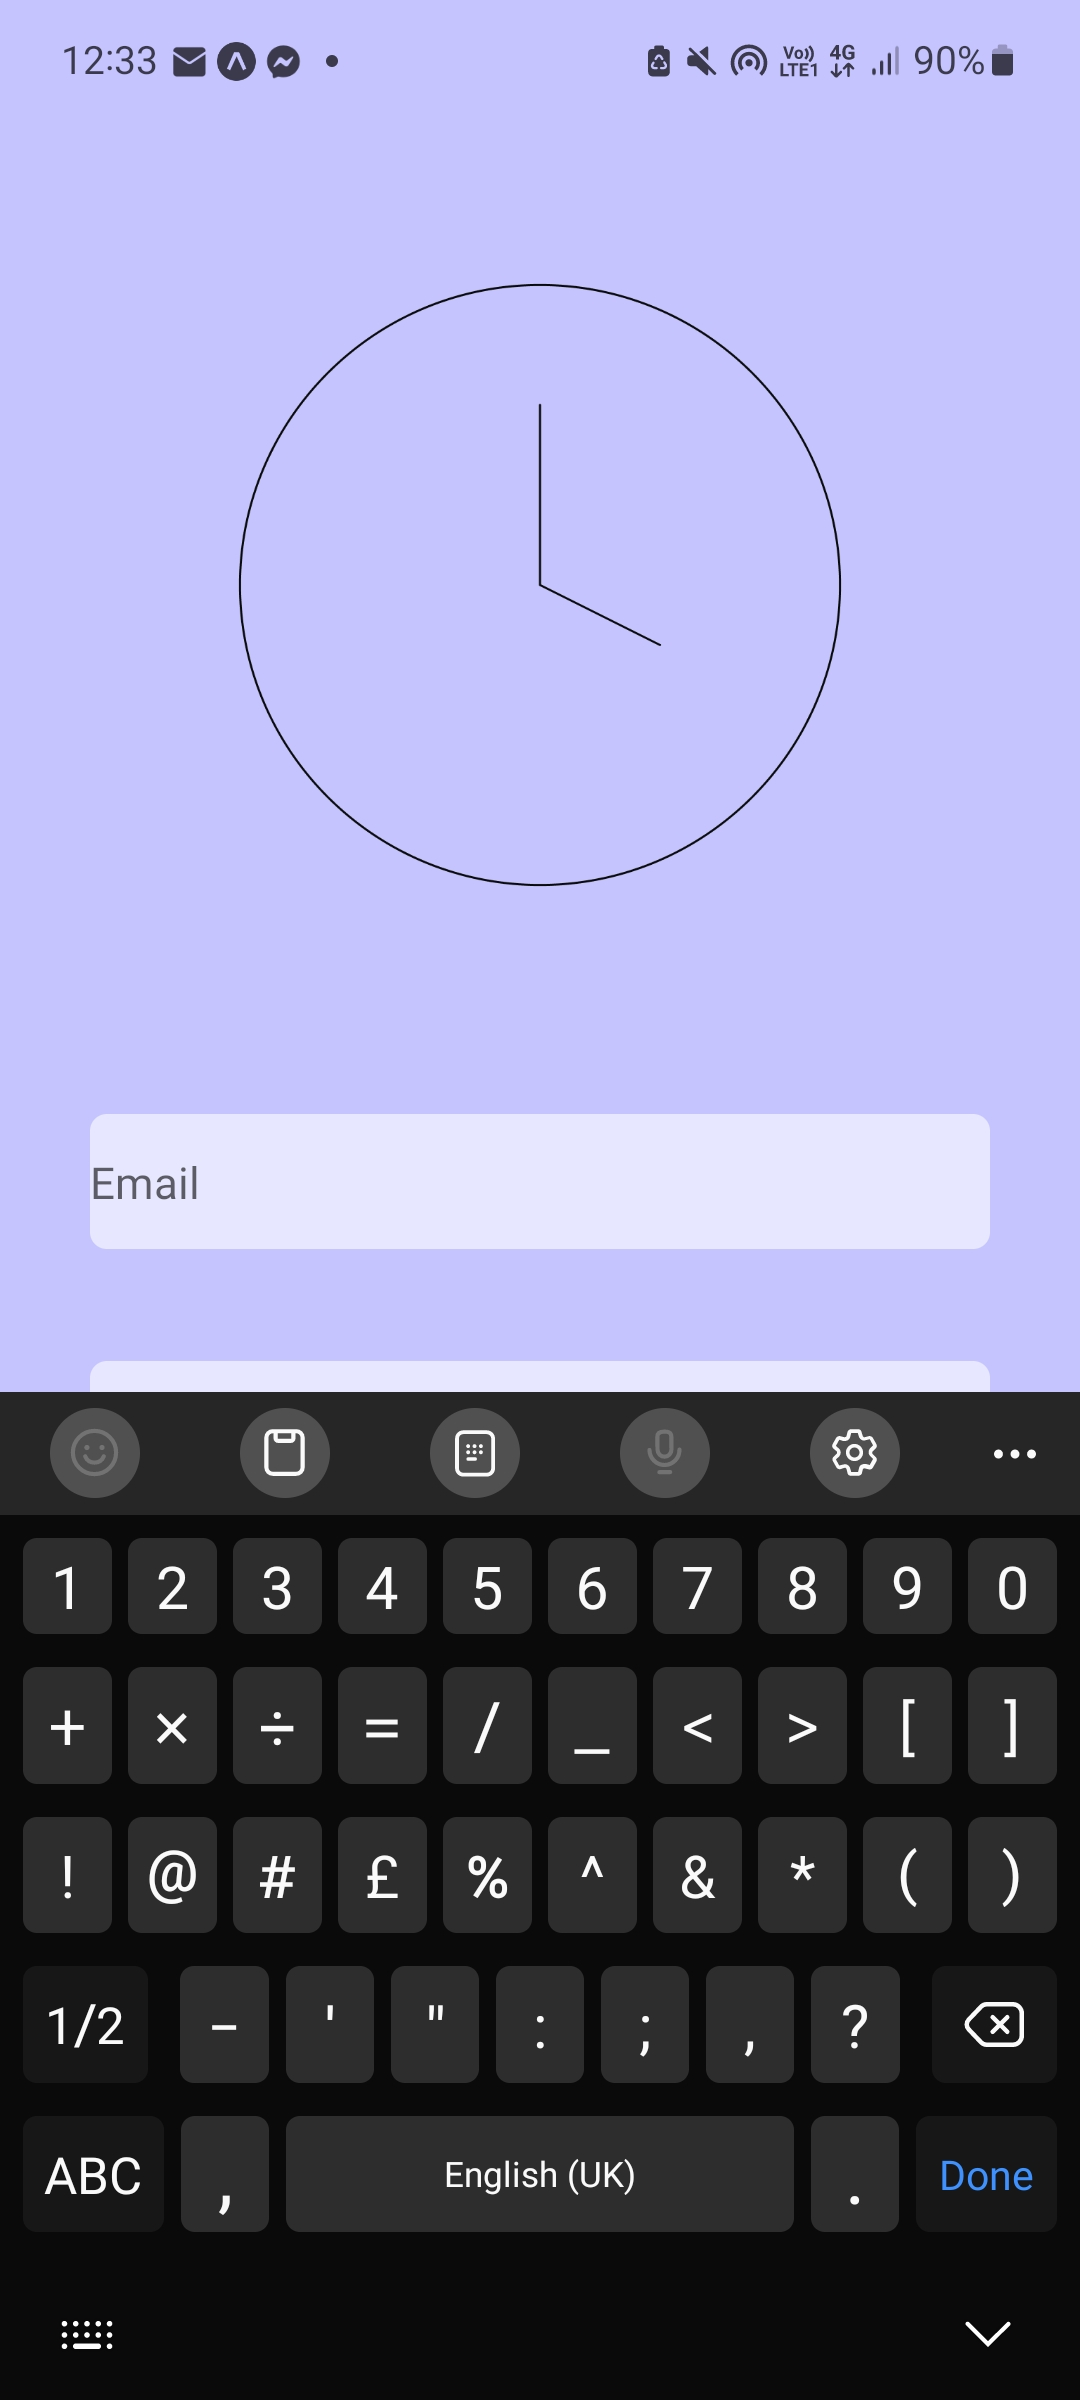
\includegraphics[width=\textwidth]{beforeKeyboard.jpg}
        \caption{\textbf{Before:} The password text input is covered by the keyboard}
    \end{subfigure}
    \hspace{1.5em}
    \begin{subfigure}[b]{0.25\textwidth}
        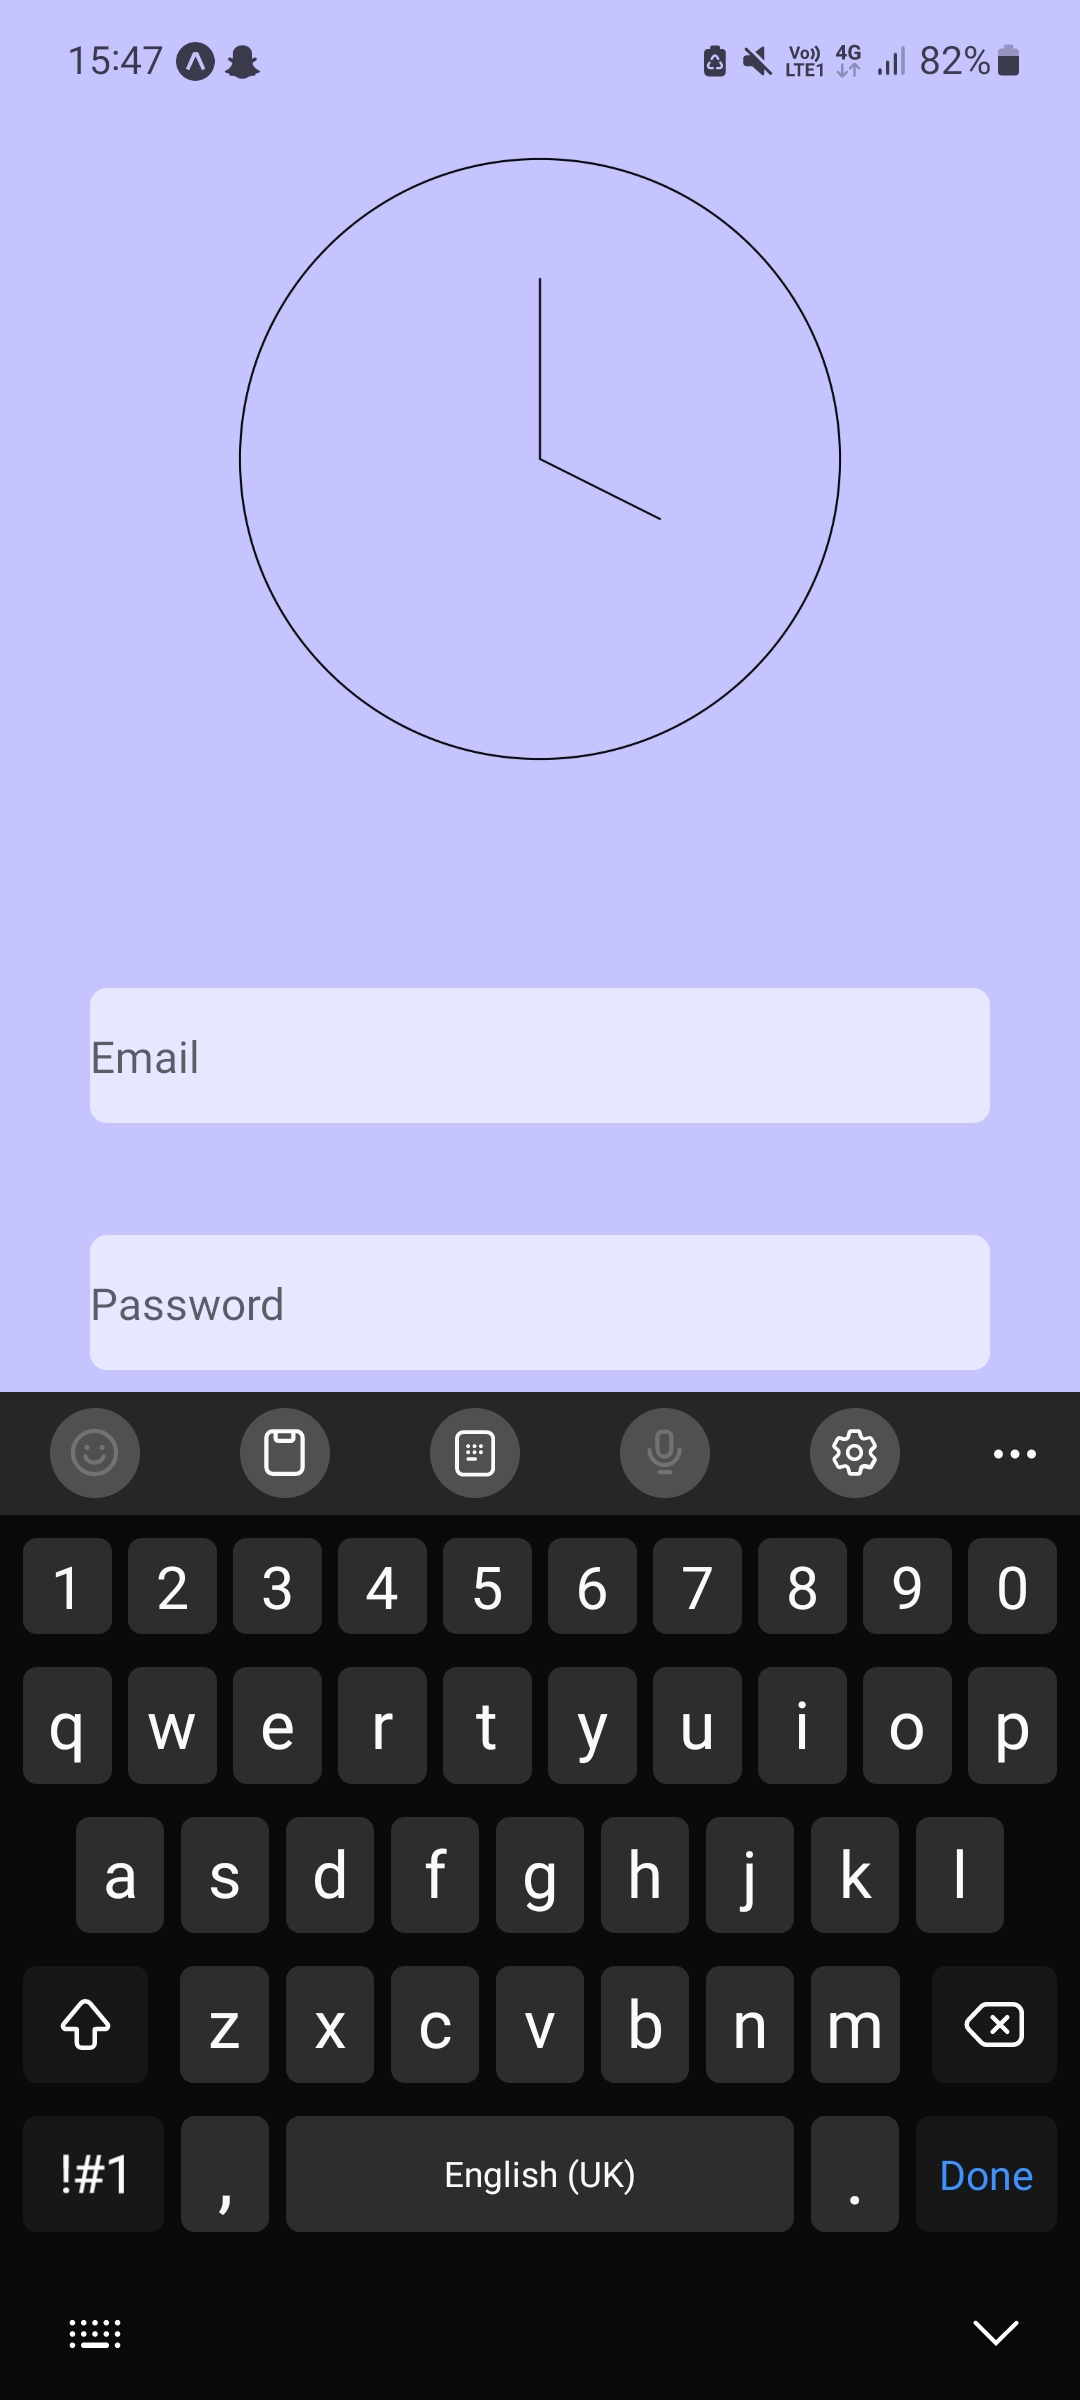
\includegraphics[width=\textwidth]{afterKeyboard.jpg}
        \caption{\textbf{After:} The screen has moved down to  allow  the user to see the password text input}
    \end{subfigure}
    \caption{Keyboard covering text entry solution }
    \label{fig:keyboard}
\end{figure}


\subsection*{Asynchronous Issues}
Interactions with the realtime database are performed through the use of an asynchronous listener to a reference to the database. For functions relying on data being previously fetched, this creates an issue. When retrieving data from the database a promise is returned, which will either resolve to the desired result or return an error. If a future function relies on this data being fetched, and we have not waited on the resolved promise, this will create problems. JavaScript provides \texttt{async}, and \texttt{await} keywords to allow the developer to create asynchronous functions, and await their promises being resolved. The use of these keywords allowed functions to wait until data had been fetched, or updated before continuing (see \ref{fig:asyncAwait}). Throughout the implementation phase, this was a constant challenge that presented itself when trying to integrate asynchronous, and synchronous code.

\begin{figure}[!htbp]
    \centering
    \begin{subfigure}[b]{0.8\textwidth}
        \begin{lstlisting}[language=jsJsx]
        onPress={async () => {
              await update(ref(db, `/users/${uid}`), {
                bio: bioNew,
              }).then(() => {
                Alert.alert("Success", "Bio changed succesfully");
                setBioModalVisible(false);
              });
        }}
        \end{lstlisting}
    \end{subfigure}
\caption{Example of awaiting the resolution of a promise from an asynchronous function}
\small\textit{The \texttt{onPress} function waits until the database has been updated with the new bio which activates the \texttt{then} method that alerts the user to the success and closes the Modal}
\label{fig:asyncAwait}
\end{figure}
\FloatBarrier

\subsection*{Rendering Issues}
An advantage of using React native is that when props or a state changes, a render occurs presenting the most up-to-date UI to the user. Whilst this is an advantage, this also creates problems when a screen is either not re-rendering to show the most up-to-date information, or is rendering too frequently. When we use state in our application for storing values, any updates to this state have the side effect of re-rendering the page unnecessarily. This can cause state within components and functions to be lost, creating unwanted problems. React Native provides a \texttt{useEffect} hook that can be used to only execute the code contained if a dependency listed has changed (see \ref{fig:useEffect}). This hook was used to control the renders of a page by only fetching data and updating state when required. Ensuring data was loaded and pages re-rendered only when necessary was a challenge dealt with throughout the entirety of the project, but made easier with the use of this hook.
\begin{figure}[!htbp]
    \centering
    \begin{subfigure}[b]{0.8\textwidth}
        \begin{lstlisting}[language=jsJsx]
        React.useEffect(() => { fetchData(); }, [isHandModalVisible]);
        \end{lstlisting}
    \end{subfigure}
\caption{Example of \texttt{useEffect} hook for controlling renders}
\small\textit{The \texttt{fetchData} function is only called when the state of \texttt{isHandModalVisible} has changed}
\label{fig:useEffect}
\end{figure}
\FloatBarrier

\section{Completion of Requirements}
The current release satisfies ten out of the thirteen functional requirements listed in \ref{functional}, with a fully functioning application delivered. Requirements were prioritised using the MoSCoW method (see \ref{reqPrior}) which allowed for the requirements crucial to the successful delivery of the application to be implemented initially, with lower priority requirements set to be implemented in the future. All four `must have', and six `should have' prioritised requirements were satisfied with these requirements being of high importance to project success. The singular `could have', and two `won't have' requirements were not met at this stage but are planned to be implemented in the future. In conclusion, all high priority requirements were satisfied with only low priority requirements left for future releases, this indicates success in the implementation of this application.


\section{Summary}

In summary, this chapter covered the implementation of the application, and the technologies used to achieve this. Github, and Git were used throughout the project as version control to keep the project organised. The front end of the application was implemented with React Native, and Tailwind CSS, creating an aesthetically pleasing, and usable application. Firebase was used to handle the storage of data, and media for the application, along with authentication used for accessing these resources. Code analysis tool ESLint, and formatter Prettier were used to ensure that the code was of a consistent style, and bug free. Many considerations for accessibility from WCAG, and Nielsen's heuristics were made to ensure the application was accessible and usable. There were many challenges faced during the implementation that are also documented such as hand placement, and rendering.